\documentclass[11pt]{article}
\usepackage[letterpaper,top=2cm,bottom=2cm,left=2cm,right=2cm,marginparwidth=1.75cm]{geometry}

 % Useful packages 
\usepackage{hyperref}
\usepackage{biblatex}
\addbibresource{Bib.bib}
\usepackage{mathtools}
\DeclarePairedDelimiterXPP\BigOSI[2]%
  {\mathcal{O}}{(}{)}{}%
  {\SI{#1}{#2}}

\usepackage{amsmath}
\usepackage{empheq}
\usepackage{amssymb}
\usepackage[most]{tcolorbox}
\usepackage{amsmath}
\usepackage{mathrsfs}
\usepackage[utf8]{inputenc}
\usepackage{graphicx}
\usepackage{float}
\usepackage{parskip}
\usepackage{comment}
\usepackage{mhchem}
 \usepackage{tabularx}
 \usepackage{titling}
  \usepackage[explicit]{titlesec}
\usepackage{fancyhdr}
\setlength{\droptitle}{3em} 

\title{Condensed Matter I}
\author{Thomas Brosnan}
\date{Notes taken in Professor Igor Shvets' class, Michaelmas Term 2023}

\tcbset{highlight math style={boxsep=2mm,,colback=blue!0!green!0!red!0!}}

  \newenvironment{bux}
    {
    \empheq[box=\tcbhighmath]{align}
   }{
    \endempheq
    }
    \newenvironment{bux*}
    {
    \empheq[box=\tcbhighmath]{align*}
   }{
    \endempheq
    }
\numberwithin{equation}{section}

\newtcbox{\mymath}[1][]{%
    nobeforeafter, math upper, tcbox raise base,
    enhanced, colframe=blue!30!black,
    colback=blue!30, boxrule=1pt,
    #1}

\newcommand{\hsp}{\hspace{8pt}}

\newcommand*{\sectionFont}{%
  \LARGE\bfseries
}

\makeatletter
\let\Title\@title % Copy the title to a new command
\makeatother

%change this RGB value to change the section background colour 
\definecolor{mycolor1}{RGB}{156, 72, 1}
\colorlet{SectionColour}{mycolor1}
%subsection background colour 
\definecolor{mycolor2}{gray}{0.8}
\colorlet{subSectionColour}{mycolor2}
%subsubsection background colour 
\definecolor{mycolor3}{RGB}{255,255,255}
\colorlet{subsubSectionColour}{mycolor3}

\begin{document}

\maketitle

\newpage

\tableofcontents
% For \section
 \titleformat{\section}[block]{\sectionFont}{}{0pt}{%
 \fcolorbox{black}{SectionColour}{\noindent\begin{minipage}{\dimexpr\textwidth-2\fboxsep-2\fboxrule\relax}\thesection  \hsp #1 {\strut} \end{minipage}}}
% For \subsection
 \titleformat{\subsection}[block]{\bfseries}{}{0pt}{%
 \fcolorbox{black}{subSectionColour}{\noindent\begin{minipage}{\dimexpr\textwidth-2\fboxsep-2\fboxrule\relax}\thesubsection  \hsp #1 {\strut} \end{minipage}}}
% For \section*
 \titleformat{name=\section, numberless}[block]{\sectionFont}{}{0pt}{%
 \fcolorbox{black}{SectionColour}{\noindent\begin{minipage}{\dimexpr\textwidth-2\fboxsep-2\fboxrule\relax} #1 {\strut} \end{minipage}}}
  % For \subsection*
 \titleformat{name=\subsection, numberless}[block]{\bfseries}{}{0pt}{%
 \fcolorbox{black}{subSectionColour}{\noindent\begin{minipage}{\dimexpr\textwidth-2\fboxsep-2\fboxrule\relax} #1 {\strut} \end{minipage}}}
 % For \subsubsection
 \titleformat{\subsubsection}[block]{\bfseries}{}{0pt}{%
 \fcolorbox{black}{subsubSectionColour}{\noindent\begin{minipage}{15cm}\thesubsubsection \hsp #1 {\strut} \end{minipage}}}
  % For \subsubsection*
 \titleformat{name=\subsubsection, numberless}[block]{\bfseries}{}{0pt}{%
 \fcolorbox{black}{subsubSectionColour}{\noindent\begin{minipage}{15cm} #1 {\strut} \end{minipage}}}
\newpage
%header 
\pagestyle{fancy}
\fancyhf{} % Clear all header and footer fields
\fancyhead[L]{\Title}
\fancyhead[R]{\nouppercase{\leftmark}}
\fancyfoot[C]{-~\thepage~-}
\renewcommand{\headrulewidth}{1pt}



\normalsize
\tcbset{highlight math style={boxsep=5mm,colback=blue!0!green!0!red!0!}}
\newpage
\section{Crystals}
\begin{itemize}
    \item Solids can be categorised into either crystalline or non-crystalline solids. In this course we will be focusing on the structures found in crystalline solids.
\end{itemize}

\subsection{Crystal definition:} 
\begin{itemize}
    \item A Crystal is a solid in which the constituent atoms, molecules or ions are packed in a regularly ordered, repeating pattern extending in all three dimensions. 

Crystals may not have macro structures that are visible to us, but a closer look at the substance will reveal a repeating pattern. 
\end{itemize}

\subsection{Spinel group}
\begin{itemize}
    \item Refers to a class of mineral with the general formulation:
\begin{empheq}[box=\tcbhighmath]{equation}
\begin{split}
   A^{2+}B^{3+}O_4^{2-}
\end{split}
\end{empheq}
The oxide anions arrange in a cubic lattice with the $A$ and $B$ cations occupying the Tetrahedral and Octahedral sites. 

In the case of Magnetite ($Fe_3O_4$) the iron is both $A$ and $B$ with a mix of $Fe^{2+}$ and $Fe^{3+}$, which results in electrons flowing between them making the material a conductor. 


\end{itemize}

\subsection{Lattice}
\begin{itemize}
    \item Is a regular, periodic array of points throughout an area or space. 
\end{itemize}

\subsection{Lattice Basis}
\begin{itemize}
    \item A lattice is the underlying pattern of the crystal. The lattice basis is then the atom(s) assigned to each point of the lattice, notably this can be more than one atom. 

More complex structures will naturally have more complex bases and the bases elements must consist of identical physical units. However the basis that is assigned to each point does not have to be located near this point, as a translation will result in the same lattice. 

As well as this our choice of basis is not unique, there are many ways we can assign atom(s) to a point. 

If a basis itself is not symmetric, it can result in the substance itself no longer being independent of the direction of measurement.
\end{itemize}

\subsection{Bravais Lattice}
\begin{itemize}
\item This is the foundation of any crystal structure. It is defined as any of these:
\item (i)An infinite array of discrete points that appear exactly the same from which ever of the points the array is viewed.
\item (ii)All the points with position:
\begin{empheq}[box=\tcbhighmath]{equation}
\begin{split}
   \textbf{R} = n_1\textbf{a}_1+n_2\textbf{a}_2+n_3\textbf{a}_3
\end{split}
\end{empheq}
Where $\textbf{a}_1,\textbf{a}_2, \textbf{a}_3$ are three vectors not in the same plane and $n_1,n_2,n_3$ integer values.
\item(iii) A discrete set of vectors (known as primitive vectors), not all in the same plane, closed under vector addition or subtraction.

The Honeycomb structure is not a bravais lattice as it does not appear the same when viewed from different points. 

\begin{figure}[H]
\centering
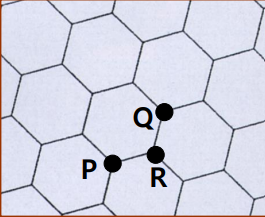
\includegraphics[width=0.5\textwidth]{Graph1.png}
\caption{\label{fig:2}\emph{Honeycomb lattice}}
\end{figure}
\item However every non bravais lattice can be created from a bravais lattice with a basis. 
\begin{figure}[H]
\centering
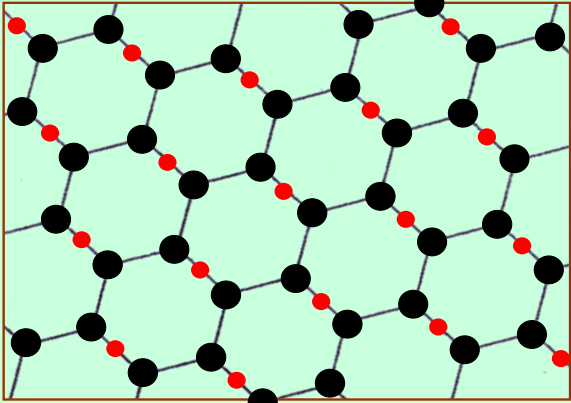
\includegraphics[width=0.5\textwidth]{Graph2.png}
\caption{\label{fig:2}\emph{Honeycomb lattice, made from Bravais lattice with a basis}}
\end{figure}
\item The choice of  primitive vectors that describe the lattice is not unique, there are infinitely many as any vector that goes from one lattice point to any other can be used as one of these vectors (as long as the don't go past other lattice points). 

Every point of the lattice can then be described as a linear combination of these primitive vectors. 


\end{itemize}

\subsection{Common Bravais Lattices}
\begin{itemize}
    \item Simple Cubic (sc)
Is one of the most familiar lattices and is common among multi-atom bases. It is easy to take the primitive vectors to be mutually orthogonal and common magnitudes. $\textbf{a}_1 = (a,0,0),\textbf{a}_2 = (0,a,0),\textbf{a}_3 = (0,0,a)$. 
\begin{figure}[H]
\centering
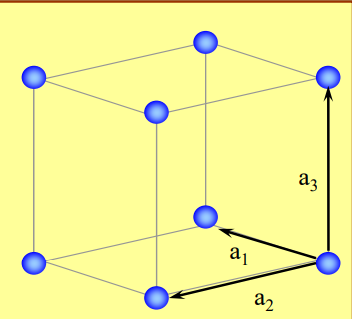
\includegraphics[width=0.5\textwidth]{Graph3.png}
\caption{\label{fig:2}\emph{Simple cubic lattice}}
\end{figure}

\item Body centered cubic (BCC)
Similar to sc but with an extra lattice point in the center of the cube. A particular choice of basis vectors for BCC is $\textbf{a}_1 = (a,0,0),\textbf{a}_2 = (0,a,0),\textbf{a}_3 = \frac{a}{2}(1,1,1) $. 
\begin{figure}[H]
\centering
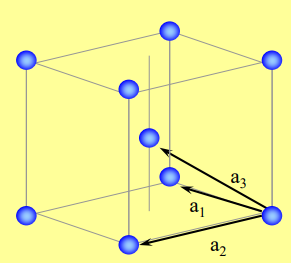
\includegraphics[width=0.5\textwidth]{image.png}
\caption{\label{fig:2}\emph{Body-Centered lattice}}
\end{figure}
\item Face centered cubic:
Instead of the extra lattice point being in the center of the cube it is now in the center of each of the faces of the cube. A symmetric choice of basis vectors is $\textbf{a}_1 = \frac{a}{2}(0,1,1),v,\textbf{a}_2 = \frac{a}{2}(1,0,1),\textbf{a}_3 = \frac{a}{2}(1,1,0)$.
\begin{figure}[H]
\centering
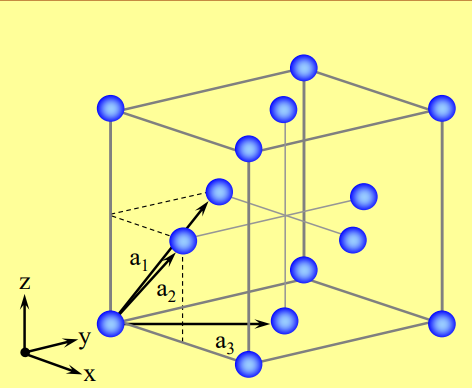
\includegraphics[width=0.5\textwidth]{Graph5.png}
\caption{\label{fig:2}\emph{Face-Centered cubic lattice}}
\end{figure}
\subsection{Simple hexagonal lattice} 
\item This is an example of a non cubic Bravais lattice.  Consists of 2D triangular (must be equilateral) nets stacked on top of each other. 
\begin{figure}[H]
\centering
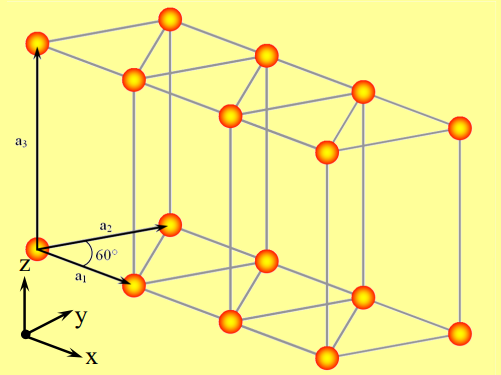
\includegraphics[width=0.5\textwidth]{Graph6.png}
\caption{\label{fig:2}\emph{Simple hexagonal lattice}}
\end{figure}
\item Primitive vectors: $\textbf{a}_1 = (a,0,0),\textbf{a}_2 = (\frac{a}{2},\frac{a\sqrt{3}}{2},0), \textbf{a}_3 = (0,0,c)$
 
\end{itemize}

\subsection{Nearest neighbours }
\begin{itemize}
    \item These are the points in a Bravais lattice that are closest to a given point.
\end{itemize}

\subsection{Coordination number}
\begin{itemize}
    \item Since Bravais lattices are periodic, each point in the lattice has the same number of nearest neighbours, we call this number the coordination number. 


\end{itemize}

\subsection{Primitive unit cell}
\begin{itemize}
    \item This is the volume that, when translated through all the vectors in a Bravais lattice just fills all space without overlapping or leaving voids.  This can be mathematically defined as:

The set of all points of the form:
\begin{empheq}[box=\tcbhighmath]{equation}
\begin{split}
   \textbf{r} = x_1\textbf{a}_1+x_2\textbf{a}_2+x_3\textbf{a}_3
\end{split}
\end{empheq}
Where the vectors $\textbf{a}_i$ are a set of primitive vectors and each $x_i$, has $0 \leq x_i  \leq 1$ .  

Each primitive cell contains just one point of the Bravais  lattice, even if there are points on its surface.  

This means that the volume $V$ is:
\begin{empheq}[box=\tcbhighmath]{equation}
\begin{split}
  V = \frac{1}{n}
\end{split}
\end{empheq}
Where $n$ is the density of points. 

Since there is no unique choice of primitive vectors there is no unique way of choosing a primitive cell.  However the volume of each choice must be the same. 

One problem with using the primitive unit cell is that it doesn't display the full symmetry of the lattice. 
\end{itemize}
\subsection{Wigner-Seitz primitive cell}
\begin{itemize}
    \item This is the region of space around a certain lattice point that is closer to that lattice. 
\end{itemize}
\subsection{Conventional unit cell}
\begin{itemize}
    \item This is the unit cell that fills up all the space with out overlapping when translated through some subset of vectors of a bravais lattice.

It is generally bigger than the primitive cell, dimensions specifying the size of the unit cell are called the lattice constants. 

Each corner lattice point is equivalent to 1/8 of a lattice point per unit cell. Similarly lattice points on the edge of a unit cell are shared among four unit cells and are worth 1/4 of a lattice point per unit cell. Lattice points on the face of a unit cell are shared between two unit cells and are worth 1/2 of a lattice point per unit cell. Lattice points contained entirely within the unit cell are worth one lattice point per unit cell.
\end{itemize}


\subsection{Symmetry group}
\begin{itemize}
    \item There are a number of operations that can act on the Bravais lattice and leave it looking unchanged. The full set of all these operations is called the symmetry group or the space group. The operations include rotations, reflections and inversions as well as of course translations. 
\end{itemize}

\subsection{Point group}
\begin{itemize}
    \item This is the set of symmetry operations on the lattice that hold one point in place while moving each remaining point to the position of another lattice point. 

It can then be proved that any symmetry operation can be broken down into a translation through a lattice vector combined with an operation from the point group. 

Thus the only type of operations on a Bravais lattice are: translations, point group operations and combinations of the two. 
\end{itemize}

\subsection{Point group operations}
\begin{itemize}
    \item There are only 5 types of point group operations:

\item 1 Rotations through integral multiples of $\frac{2\pi}{n}$ about some axis (for an $n$-fold rotational axis). 

\item 2 Rotation + Reflection, a rotation through $\frac{2\pi}{n}$ that is not a symmetry element may be made a symmetric by following the rotation with a reflection, in a plane perpendicular to the axis. 

\item 3 Rotation+inversions, similar to the above a rotation that is not symmetric can be followed by an inversion to make it so. 

\item 4 Reflections themselves are also symmetry operations.

\item 5 Inversions, a single point remains fixed and every other point given by a vector $\textbf{r}$ compared to the fixed point, is taken to $-\textbf{r}$. 
\end{itemize}

\subsection{Crystal systems}
\begin{itemize}
    \item Crystal structures can be categorised into one of the seven crystal systems, each one corresponding to a different point group. These crystal systems are based on the underlying symmetries of the Bravais lattice. 
\end{itemize}


\begin{figure}[H]
\centering
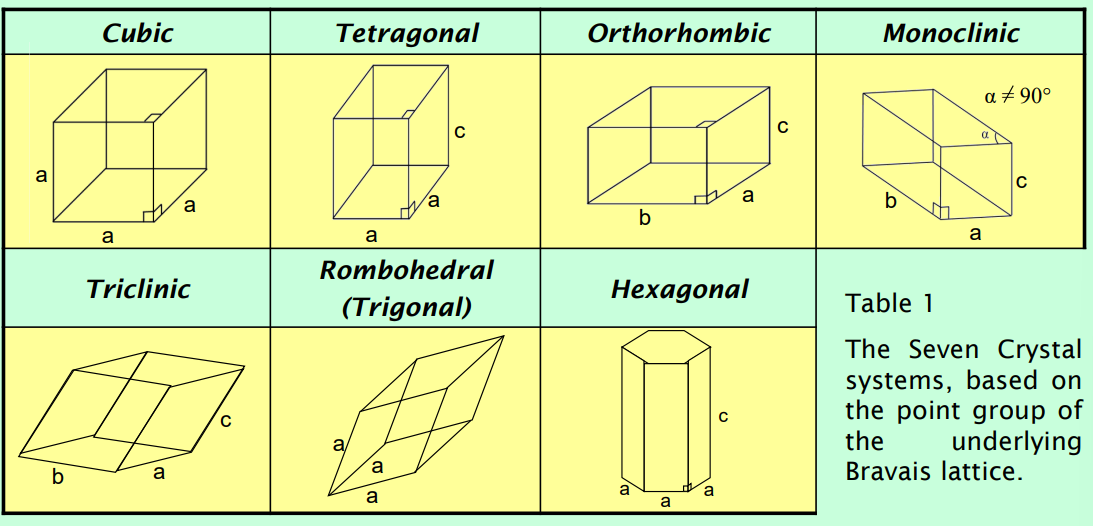
\includegraphics[width=0.7\textwidth]{Graph7.png}
\caption{\label{fig:2}\emph{Seven crystal systems}}
\end{figure}
\subsection{Bravais space groups }
\begin{itemize}
    \item When considering the full symmetry groups there are fourteen distinct space groups: 
\begin{figure}[H]
\centering
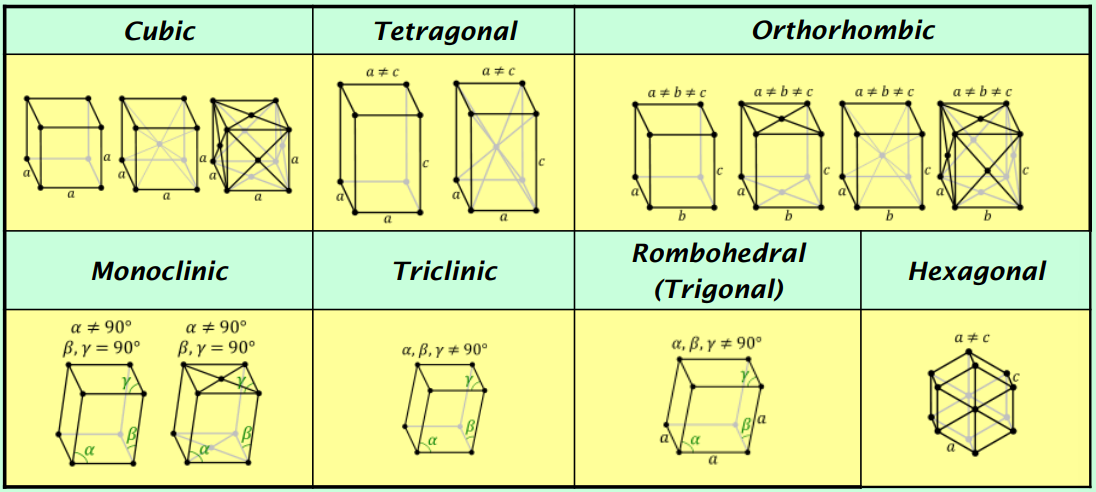
\includegraphics[width=0.7\textwidth]{Graph8.png}
\caption{\label{fig:2}\emph{14 space groups}}
\end{figure}
\end{itemize}

\subsection{Fourier analysis of a crystal structure}
\begin{itemize}
    \item A crystal structure with a Bravais lattice is invariant under any translations $\textbf{T}$ of integer multiples of their primitive vectors. Thus physical properties of the crystal can be described using periodic functions. $f(\textbf{r}+ \textbf{T}) = f(\textbf{r})$. This allows us to write functions with a period $a$ as a Fourier series:
\begin{empheq}[box=\tcbhighmath]{equation}
\begin{split}
 f(x) = f_0 = \sum_{j=1}^{\infty}A_j \cos(\frac{2\pi j x}{a}) + \sum_{j=1}^{\infty}B_j \sin(\frac{2\pi j x}{a}) = \sum_{j=-\infty}^{j=\infty} C_je^{\frac{2i\pi jx}{a}}
\end{split}
\end{empheq}


\end{itemize}

\subsection{Reciprocal Space}
\begin{itemize}
    \item Also called the k space, this is space in which the Fourier transform of a spatial function is represented. 
\end{itemize}


\subsection{Reciprocal Lattice}
\begin{itemize}
    \item We say $\frac{2 \pi j}{a}$ forms a set of points in the 1D reciprocal lattice of the crystal. 

In 3D the points become 3 dimensional vectors. These vectors $\textbf{k}$ are called wave vectors, which yield plane waves with the same periodicity of the Bravais Lattice. 

If we have a Bravais lattice consisting of all points $\textbf{R}$ and a plane wave defined by the wave vector $\textbf{k}$, then since:
\begin{bux}
\begin{split}
e^{i\textbf{k}\cdot(\textbf{r}+\textbf{R})} = 
e^{i\textbf{k}\cdot\textbf{r}}e^{i\textbf{k}\cdot\textbf{R}}  = e^{i\textbf{k}\cdot\textbf{r}}  \implies \textbf{k}\cdot \textbf{R} = 2 \pi p, ~~p \in \mathbb{Z}
\end{split}
\end{bux}

Every crystal structure has two lattices associated with it, crystal lattice and reciprocal lattice. The two lattices primitive vectors are related by:
\begin{empheq}[box=\tcbhighmath]{equation}
\begin{split}
\textbf{b}_1 = 2 \pi \frac{\textbf{a}_2\times \textbf{a}_3}{\textbf{a}_1\cdot(\textbf{a}_2\times \textbf{a}_3)},~~~\textbf{b}_2 = 2 \pi \frac{\textbf{a}_3\times \textbf{a}_1}{\textbf{a}_1\cdot(\textbf{a}_2\times \textbf{a}_3)},~~~\textbf{b}_3 = 2 \pi \frac{\textbf{a}_1\times \textbf{a}_2}{\textbf{a}_1\cdot(\textbf{a}_2\times \textbf{a}_3)}
\end{split}
\end{empheq}
The reciprocal of the reciprocal is the original lattice. We also have that:
\begin{empheq}[box=\tcbhighmath]{equation}
\begin{split}
\textbf{b}_i \cdot \textbf{a}_j = 2 \pi \delta_{ij}
\end{split}
\end{empheq}


\item If the volume of the primitive cell in the direct lattice is given by $V$ then the volume of the primitive cell in the reciprocal lattice is $V' = \frac{(2 \pi )^3}{V}$. 

The Wigner-Seitz primitive cell of the reciprocal lattice is known as the Brillouin zone.





\end{itemize}

\subsection{Packing  fraction}
\begin{itemize}
    \item This is the ratio of the volume of the largest spheres surrounding each lattice point such that they don't overlap, in a unit cell, to the volume of this unit cell. 
\begin{empheq}[box=\tcbhighmath]{equation}
\begin{split}
PF = \frac{N_{lattice~points}V_{Sphere}}{V_{unit~cell}}
\end{split}
\end{empheq}

\end{itemize}
\subsection{Lattice planes}
\begin{itemize}
    \item Is defined to be any plane containing at least three non-collinear lattice points.  because of translational symmetry this plane will contain infinite number of lattices points, which in turn form a two-dimensional Bravais lattice. 

\item A family of lattice planes is a set of parallel equally spaced planes which together contain all the points of a 3D Bravais lattice. Any lattice plane is a member of one such family.  
\end{itemize}

\subsection{Reciprocal vectors and lattice planes}
\begin{itemize}
    \item For any family of lattice planes separated by a distance $d$, there are reciprocal lattice vectors perpendicular to the planes, the shortest of which has a length $2 \pi/ d$. 

Conversely, for any reciprocal lattice vector $\textbf{k}$, there is a family of lattice planes normal to $\textbf{k}$ and separated by  a distance $d$, where $2 \pi/ d$ is the length of the shortest lattice vector parallel to $\textbf{k}$. 
\end{itemize}

\subsection{Miller indices}
\begin{itemize}
    \item The Miller indices of a lattice plane are the coordinates of the shortest reciprocal lattice vector normal to that plane with respect to a specified set of primitive reciprocal lattice vectors. 

Thus a plane with miller indices $h,k,l$ is normal to the reciprocal lattice vector $h \textbf{b}_1 + k \textbf{b}_2 + l \textbf{b}_3$. From this very definition we know the Miller indices $h,k,l$ must have integer values.  
\end{itemize}

\begin{itemize}
    \item In crystallography there are conventions as to how the indices of planes and directions are written. When referring to a specific plane, “round” brackets are used:  $(hkl)$.  If one of  the indices is negative it is replaced with a bar over it instead of a minus sign.

Vectors written in terms of multiples of the lattice vectors $a_1$ , $a_2$ , and $a_3$ are directions in the crystal written with “square” brackets: $[UVW]$. 

A number of crystallographic directions can also be symmetrically equivalent, in which case a set of directions are written with “triangular” brackets:  $<UVW>$. 
\end{itemize}






\end{document}
